\documentclass{beamer}

\definecolor{theme}{RGB}{28,90,127}
\definecolor{offblack}{HTML}{262626}
\setbeamercolor{normal text}{fg=offblack}

\usecolortheme[named=theme]{structure}
\usecolortheme{dolphin}  % outer color theme
\usecolortheme{orchid}  % inner color theme

% modified version of default frametitle with horizontal separation line
\makeatletter
\setbeamertemplate{frametitle}{
  \ifbeamercolorempty[bg]{frametitle}{}{\nointerlineskip}%
  \@tempdima=\textwidth%
  \advance\@tempdima by\beamer@leftmargin%
  \advance\@tempdima by\beamer@rightmargin%
  \begin{beamercolorbox}[sep=0.3cm,left,wd=\the\@tempdima]{frametitle}
    \usebeamerfont{frametitle}%
    \vbox{}\vskip-2ex%
    \if@tempswa\else\csname beamer@fteleft\endcsname\fi%
    \strut\insertframetitle\strut\par%
    {%
      \ifx\insertframesubtitle\@empty%
      \else%
      {\usebeamerfont{framesubtitle}\usebeamercolor[fg]{framesubtitle}\insertframesubtitle\strut\par}%
      \fi
    }%
    \vskip.45ex%
    \hrule %height .6pt%
    \vskip-1.45ex%
    \if@tempswa\else\vskip-.3cm\fi%
  \end{beamercolorbox}%
}
\makeatother

% clean up footer
\beamertemplatenavigationsymbolsempty
\beamertemplatenavigationsymbolsempty
\defbeamertemplate{footline}{custom footline}{
  \usebeamercolor[fg]{page number in head/foot}
  \usebeamerfont{page number in head/foot}
  \quad
  \insertauthor\enskip(\insertshortinstitute)
  \hskip 7em
  \insertshorttitle
  \hfill
  \insertframenumber\,/\,\inserttotalframenumber\kern1em\vskip2pt
}
\setbeamertemplate{footline}[custom footline]

\useinnertheme{default}
\setbeamertemplate{itemize item}{\raise.35ex\hbox{\vrule width .7ex height .7ex}}
\setbeamertemplate{itemize subitem}{\raise.35ex\hbox{\vrule width .6ex height .6ex}}

% for backup slides
\usepackage{appendixnumberbeamer}

\usepackage{graphicx}
\graphicspath{{fig/}}

\usepackage{amsmath}
\usepackage{amssymb}
\usepackage{booktabs}
\usepackage{tikz}
\usetikzlibrary{matrix}

\newcommand{\avg}[1]{\langle #1 \rangle}
\newcommand{\nch}{N_\text{ch}}
\newcommand{\vnk}[2]{v_#1\{#2\}}
\newcommand{\tran}{^\intercal}
\newcommand{\trento}{T\raisebox{-.5ex}{R}ENTo}
\newcommand{\order}[1]{$\mathcal O(10^{#1})$}
\newcommand{\x}{\mathbf x}
\newcommand{\y}{\mathbf y}
\newcommand{\z}{\mathbf z}
\newcommand{\xs}{\x_\star}
\newcommand{\zs}{\z_\star}
\newcommand{\yexp}{\y_\text{exp}}
\newcommand{\zexp}{\z_\text{exp}}

\title
[Quantifying QGP properties through model-to-data comparison]
{Quantifying properties of hot and dense QCD matter through systematic model-to-data comparison}
\author{Jonah Bernhard}
\institute[Duke]{Duke University}


\begin{document}


\section{Title}

\begin{frame}[plain,noframenumbering]
  \centering
  \linespread{1.3}

  \vskip1em

  \large
  \color{theme}
  \parbox{.9\textwidth}{\centering\inserttitle}

  \vskip2em
  \color{theme}
  \hrule
  \vskip2em

  \small
  \color{offblack}
  \insertauthor \\
  \vskip1em
  \scriptsize
  INT workshop: Correlations and fluctuations in p+A and A+A collisions \\
  Tuesday, July 14, 2015

  \tikz[remember picture, overlay]
    \node[text width=\textwidth, anchor=south west, inner sep=1em]
        at (current page.south west) {
      \tiny
      \color{offblack}
      J.~E.~Bernhard, P.~W.~Marcy, C.~E.~Coleman-Smith, \\
      S.~Huzurbazar, R.~L.~Wolpert, and S.~A.~Bass, \\
      PRC \textbf{91}, 054910 (2015), arXiv:1502.00339 [nucl-th]. \\
    };
\end{frame}


\section{Introduction}


\begin{frame}{Model-to-data comparison}
  \centering
  \def\tw{\textwidth}
  \vspace{.02\tw}
  \begin{tikzpicture}[semithick]
    \def\pw{.30\tw}
    \def\dx{.55\tw}
    \def\dy{.26\tw}
    \node (lhc) {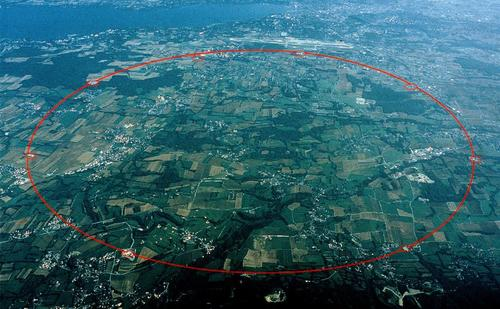
\includegraphics[width=\pw]{third_party/lhc}};
    \node[below of=lhc, node distance=\dy] (expevent)
      {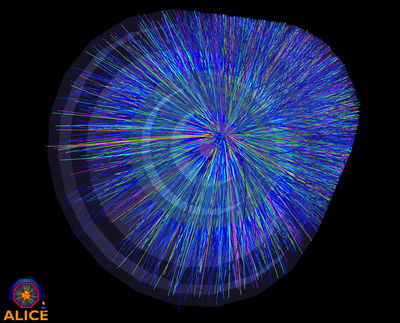
\includegraphics[width=.25\tw]{third_party/alice_event}};
    \node[below of=expevent, node distance=\dy] (expdata)
      {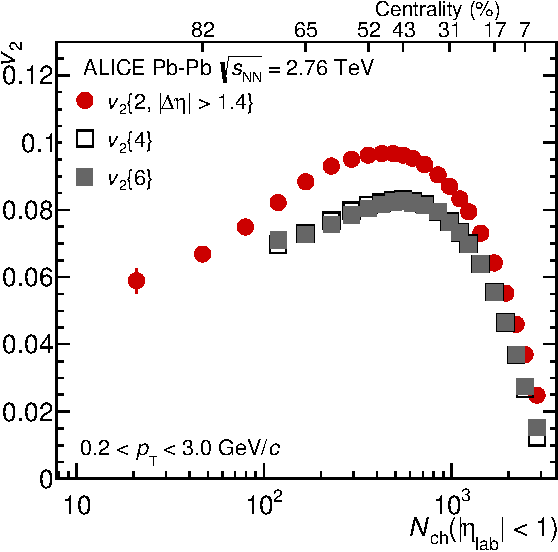
\includegraphics[width=.22\tw]{third_party/alice_data}};
    \node[right of=lhc, node distance=\dx, draw, thin,
          text width=\pw, text centered, inner sep=1ex] (modelinput)
      {\textbf{Model} \\ Initial conditions, \\ $\tau_0$, $\eta/s$, \ldots};
    \node[right of=expevent, node distance=\dx, draw, thin,
          text width=\pw, text centered, inner sep=1ex] (modelevo) {
        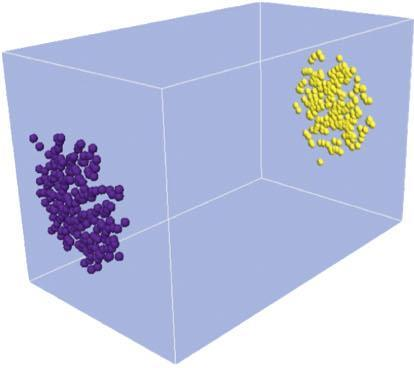
\includegraphics[width=.33\tw]{third_party/evolution1}
        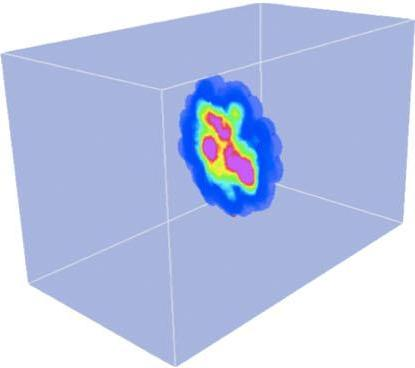
\includegraphics[width=.33\tw]{third_party/evolution2}
        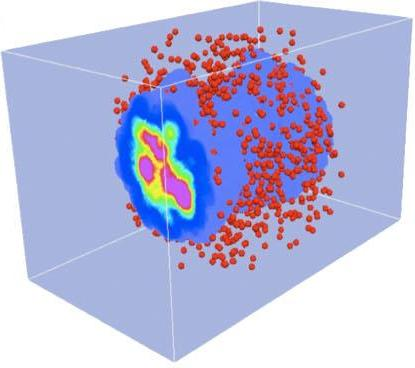
\includegraphics[width=.33\tw]{third_party/evolution3} \\
        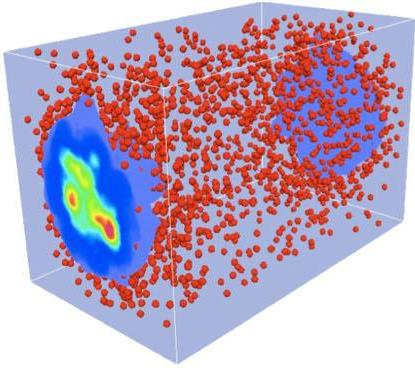
\includegraphics[width=.33\tw]{third_party/evolution4}
        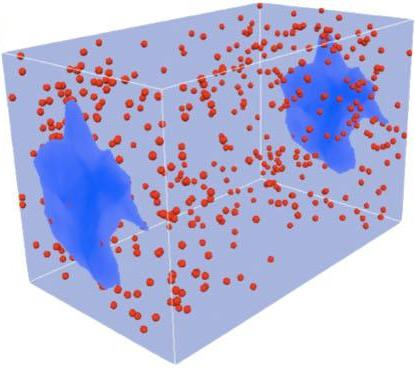
\includegraphics[width=.33\tw]{third_party/evolution5}
      };
    \node[right of=expdata, node distance=\dx, draw, thin] (modeldata)
      {\includegraphics[width=.38\tw]{prior_draws}};
    \path[->] (lhc)        edge (expevent)
              (expevent)   edge (expdata)
              (modelinput) edge (modelevo)
              (modelevo)   edge (modeldata);
    \draw[densely dashed,<->] (expdata) -- coordinate (midpt) (modeldata);
    \draw[densely dashed,->] (midpt) |- (modelinput);
  \end{tikzpicture}
\end{frame}


\begin{frame}{Measuring QGP $\eta/s$}
  \begin{enumerate}
    \item Observe experimental flow coefficients $v_n$
    \item Run model with variable $\eta/s$ \\
    \item Constrain $\eta/s$ by matching $v_n$
  \end{enumerate}
  \medskip
  \centering
  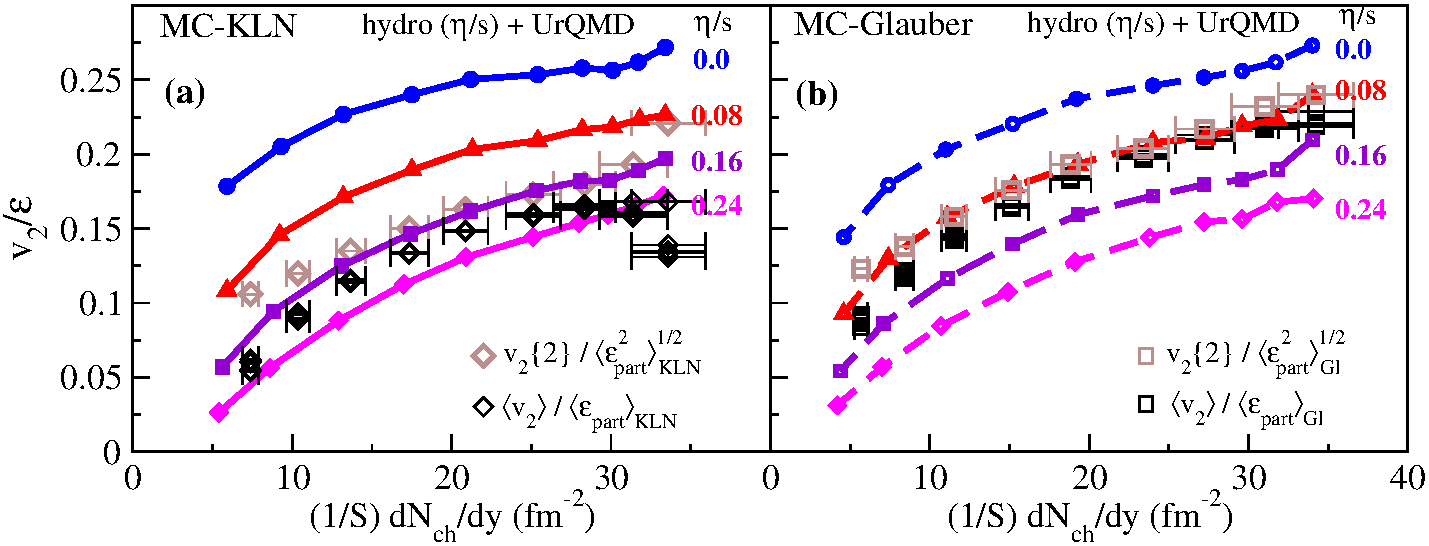
\includegraphics[width=\textwidth]{third_party/osu}
  \flushright
  \tiny
  H.~Song, S.~A.~Bass, U.~Heinz, T.~Hirano, and C.~Shen, \\
  PRL\ {\bf 106}, 192301 (2011), arXiv:1011.2783 [nucl-th].
\end{frame}


\begin{frame}{Extracting QGP properties}
  \vspace{1em}
  \begin{columns}
    \column{.45\textwidth}
    \begin{center}
      \bf Older work
    \end{center}
    \vspace{-1ex}
    \begin{itemize}
      \item Average calculations
      \item Single parameter and observable ($\eta/s \leftrightarrow v_2$)
      \item Several discrete values
      \item Qualitative constraints lacking uncertainty
    \end{itemize}

    \column{.50\textwidth}
    \begin{center}
      \bf New projects
    \end{center}
    \vspace{-1ex}
    \begin{itemize}
      \item Event-by-event model
      \item Multiple parameters \\ and observables
      \item Continuous parameter space
      \item Quantitative constraints including uncertainty
    \end{itemize}
  \end{columns}

  \vspace{2em}
  \tiny
  See also, e.g.: \\
  \begin{itemize}
    \item J.~Novak, K.~Novak, S.~Pratt, C.~Coleman-Smith, and R.~Wolpert, \\
      PRC \textbf{89}, 034917 (2014), arXiv:1303.5769 [nucl-th].
    \item R.~A.~Soltz, I.~Garishvili, M.~Cheng, B.~Abelev, A.~Glenn, J.~Newby, L.~A.~Linden Levy, and S.~Pratt, \\
      PRC {\bf 87}, 044901 (2013), arXiv:1208.0897 [nucl-th].
    \item  S.~Pratt, E.~Sangaline, P.~Sorensen,  and H.~Wang, \\
      PRL {\bf 114}, 202301 (2015), arXiv:1501.04042 [nucl-th].
  \end{itemize}

  \tikz[overlay,remember picture]
    \node[xshift=-3ex,yshift=10ex] at (current page.center)
    {$\color{theme}\Large\boldsymbol\longrightarrow$};
\end{frame}


\section{Method}

\begin{frame}{Strategy}
  \begin{enumerate}
    \item Choose set of salient model parameters
      \begin{itemize}
        \item physical properties
        \item model nuisance parameters
      \end{itemize}
    \item Run model at small $\mathcal O(10^1$--$10^2)$ set of parameter points
    \item Interpolate with Gaussian process emulator \\
      $\rightarrow$ fast stand-in for actual model
    \item Systematically explore parameter space using Bayes' theorem and Markov chain Monte Carlo (MCMC)
    \item Calibrate model emulator to optimally reproduce data \\
      $\rightarrow$ extract probability distributions for each parameter
  \end{enumerate}
\end{frame}


\begin{frame}{Event-by-event model}
    \begin{itemize}
      \item MC-Glauber \& MC-KLN initial conditions \\
        \quad {\tiny H.-J.\ Drescher and Y.\ Nara, PRC {\bf 74}, 044905 (2006).}
        \smallskip
      \item Viscous 2+1D hydro \\
        \quad {\tiny H.\ Song and U.\ Heinz, PRC {\bf 77}, 064901 (2008).}
        \smallskip
      \item Cooper-Frye hypersurface sampler \\
        \quad {\tiny C.~Shen, Z.~Qiu, H.~Song, J.~Bernhard, S.~Bass, and U.~Heinz, arXiv:1409.8164 [nucl-th].}
        \smallskip
      \item UrQMD \\
        \quad {\tiny S.\ Bass \emph{et.\ al.}, Prog.\ Part.\ Nucl.\ Phys.\  {\bf 41}, 255 (1998).} \\[-1ex]
        \quad {\tiny M.\ Bleicher \emph{et.\ al.}, J.\ Phys.\ G {\bf 25}, 1859 (1999).}
    \end{itemize}
\end{frame}


\begin{frame}{Calibration parameters}
  Initial condition parameters:
  \begin{itemize}
    \item Overall normalization factor
    \item $\alpha$ (Glauber), $\lambda$ (KLN) \\
      $\rightarrow$ both control centrality dependence of multiplicity
  \end{itemize}
  \medskip
  Hydro parameters:
  \begin{itemize}
    \item Thermalization time $\tau_0$
    \item Specific shear viscosity $\eta/s$
    \item Shear relaxation time $\tau_\pi = 6k_\pi\eta/(sT)$ \enskip [vary $k_\pi$]
  \end{itemize}
\end{frame}


\begin{frame}{Computer experiment design}
  \begin{columns}
    \column{.5\textwidth}
    Latin-hypercube design:
    \begin{itemize}
      \item Semi-randomized, space-filling points
      \item Avoids large gaps and tight clusters
      \item All parameters varied simultaneously
      \item Needs only $m \gtrsim 10n$ points
    \end{itemize}
    \smallskip
    This work:
    \begin{itemize}
      \item $m = 256$ points across $n = 5$ dimensions
      \item \order 4 events per point
    \end{itemize}

    \column{.5\textwidth}
    \small
    Design projected into $(\tau_0, \eta/s)$ dimensions: \\[1em]
    \includegraphics{design}
  \end{columns}
\end{frame}


\begin{frame}{Training data}
  \bigskip
  \centering
  Model calculations at each parameter point \\
  \bigskip
  \includegraphics{prior_draws}
  \flushright
  \tiny
  Data points: ALICE Collaboration, Pb-Pb collisions at $\sqrt{s_\text{NN}} = 2.76$ TeV \\
  B.~B.~Abelev {\it et al.}, PRC {\bf 90}, 054901 (2014), arXiv:1406.2474 [nucl-ex].
\end{frame}


\begin{frame}{Gaussian process emulator}
  \vspace{1em}
  \begin{columns}[c]
    \column{.58\textwidth}
    Gaussian process:
    \begin{itemize}
      \item Stochastic function: maps inputs to normally-distributed outputs
      \item Specified by mean and covariance functions
    \end{itemize}
    \bigskip
    As a model emulator:
    \begin{itemize}
      \item Non-parametric interpolation
      \item Predicts \emph{probability distributions}
        \begin{itemize}
          \item Narrow near training points, \\ wide in gaps
        \end{itemize}
      \item Fast ``surrogate'' to actual model
    \end{itemize}
    \column{.45\textwidth}
    \includegraphics{gp}
  \end{columns}
\end{frame}


\begin{frame}{Multivariate output}
  \begin{columns}[t]
    \column{.5\textwidth}
    Model outputs $(\nch, v_2, v_3)$ \\
    $\rightarrow$ independent emulators?
    \begin{itemize}
      \item Neglects correlations
      \item What if 100 outputs?
    \end{itemize}
    \medskip
    Principal components:
    \begin{itemize}
      \item Linear combinations of model output data
      \item Orthogonal and uncorrelated
    \end{itemize}
    \medskip
    $\rightarrow$ Emulate each PC
    \column{.5\textwidth}
    \small
    PC decomposition of $\nch$ and $v_2$ data in one centrality bin: \\[1ex]
    \includegraphics{pc_scatter}
  \end{columns}
  \medskip
  $\nch$~:~$v_2$~:~$v_3$ weighted 1.2~:~1.0~:~0.6 \\
  $\rightarrow$ encodes relative importance of describing each observable
\end{frame}


\begin{frame}{Validation}
  \begin{itemize}
    \item Independent set of validation points
    \item Run model and predict output with emulator at each point
    \item Accurate predictions fall on diagonal line
  \end{itemize}
  \medskip
  \includegraphics{validation} \\[1em]
  \scriptsize
  \hspace{2em} Horizontal error bars: $2\sigma$ emulator uncertainty \\
  \hspace{2em} Vertical error bars: $2\sigma$ statistical uncertainty
\end{frame}


\begin{frame}{Calibration}
  Input parameters:
  \begin{equation*}
    \x = (\text{Norm}, \text{I.C.\ param}, \tau_0, \eta/s, k_\pi)
  \end{equation*}
  Assume true parameters $\xs$ exist $\rightarrow$ find probability dist.\ for $\xs$ \\[1.5ex]
  Bayes' theorem:
  \begin{equation*}
    P(\xs|X,Y,\yexp) \propto P(X,Y,\yexp|\xs) P(\xs)
  \end{equation*}
  \vskip -1.5ex
  \begin{itemize}
    \item $P(\xs)$ = prior \\
      $\rightarrow$ initial knowledge of $\xs$
    \item $P(X,Y,\yexp|\xs)$ = likelihood \\
      $\rightarrow$ prob.\ of observing $(X, Y, \yexp)$ given proposed $\xs$
      \color{theme!80!black}
    \item $P(\xs|X,Y,\yexp)$ = posterior \\
      $\rightarrow$ prob.\ of $\xs$ given observations $(X, Y, \yexp)$
  \end{itemize}
\end{frame}


\begin{frame}{Markov chain Monte Carlo (MCMC)}
  \begin{itemize}
    \item Random walk through parameter space weighted by posterior
    \item Large number of samples \\
      $\rightarrow$ chain equilibrates to posterior distribution
      \bigskip
    \item Flat prior within design range, zero outside
    \item Likelihood:
      \begin{equation*}
        \log P(X,Y,\yexp|\xs) \sim -\frac{(\y_\star - \y_\text{exp})^2}{2\sigma^2}
      \end{equation*}
      $\sigma = 0.06$ on principal components (includes correlations)
    \item Posterior = likelihood within design range, zero outside
  \end{itemize}
\end{frame}


\section{Results}

\begin{frame}{$\eta/s$ posteriors}
  \begin{itemize}
    \item
      \parbox{3.5em}{Glauber}
      \parbox{5em}{$\eta/s \sim 0.06$,}
      95\% C.I.\ $\sim$ 0.02--0.10
    \item
      \parbox{3.5em}{KLN}
      \parbox{5em}{$\eta/s \sim 0.16$,}
      95\% C.I.\ $\sim$ 0.12--0.21
  \end{itemize}
  \medskip
  \centering
  \includegraphics{post_compare}
\end{frame}


% \begin{frame}[plain,noframenumbering]
%   \centering
%   \LARGE
%   Posterior distributions
% \end{frame}


\begin{frame}[plain]
  \vspace{.5ex}
  \centering
  \includegraphics{cal_post_glb}
  \tikz[remember picture, overlay]
    \node[color=gray, rotate=45, yshift=-3em] at (current page.north west)
    {Glauber};
\end{frame}


\begin{frame}[plain]
  \vspace{.5ex}
  \centering
  \includegraphics{cal_post_kln}
  \tikz[remember picture, overlay]
    \node[color=gray, rotate=45, yshift=-3em] at (current page.north west)
    {KLN};
\end{frame}


\begin{frame}{Posterior samples}
  \centering
  \bigskip
  \only<1>{
    Model calculations over full design space \\[3ex]
    \includegraphics{prior_draws}
  }
  \only<2>{
    Emulator predictions from calibrated posterior \\[3ex]
    \includegraphics{post_draws}
  }
\end{frame}


\begin{frame}{Sensitivity}
  \begin{enumerate}
    \item Go to posterior mean
    \item Vary one parameter at a time; keep others fixed at mean
    \item Emulate response of each observable
  \end{enumerate}
  \smallskip
  \centering
  Effect of $\eta/s$ on $v_2$ \\[1.5ex]
  \includegraphics{sensitivity_compare} \\
  \smallskip
  \tiny
  $x$ point = posterior mean $\pm$ 1$\sigma$ C.I., $y$ point = ALICE value
\end{frame}


\begin{frame}[plain]
  \vspace{.5ex}
  \hspace*{-.06\textwidth}
  \includegraphics{sensitivity_glb}
  \tikz[remember picture, overlay]
    \node[color=gray, rotate=90, anchor=north, xshift=4.5em] at (current page.west)
    {Glauber};
\end{frame}


\begin{frame}[plain]
  \vspace{.5ex}
  \hspace*{-.06\textwidth}
  \includegraphics{sensitivity_kln}
  \tikz[remember picture, overlay]
    \node[color=gray, rotate=90, anchor=north, xshift=4.5em] at (current page.west)
    {KLN};
\end{frame}


\section{Conclusion}

\begin{frame}{Summary}
  Framework for quantitative, systematic parameter extraction \\ and model evaluation
  \medskip
  \begin{itemize}
    \itemsep 2ex
    \item Gaussian process emulator accurately predicts model output
    \item MCMC gives full probability distributions for all parameters
    \item Glauber approximately describes $\nch$, $v_2$, $v_3$
    \item KLN cannot simultaneously fit $v_2$, $v_3$
  \end{itemize}
\end{frame}


\begin{frame}{Version 2.0}
  \begin{itemize}
    \itemsep 1ex
    \item Parametric initial condition models
      \begin{itemize}
        \item \trento\ (see Scott Moreland's talk tomorrow)
        \item fluctuated Glauber
      \end{itemize}
    \item More input parameters: nucleon size, \\ temperature-dependent $\eta/s$, bulk viscosity, \\ hydro-to-UrQMD switching temperature
    \item More observables: $\avg{p_T}$, $\vnk 2 4$, identified particles, HBT
    \item RHIC and LHC
    \item Improve treatment of uncertainty
      \medskip
    \item Eventually: simultaneous calibration to small systems
  \end{itemize}
\end{frame}


\appendix


\begin{frame}{Gaussian processes}
  \begin{definition}
    A Gaussian process is a collection of random variables, any finite number of which have a joint Gaussian distribution.
  \end{definition}
  \medskip
  Stochastic function: $\x \rightarrow y$ \\
  \begin{itemize}
    \item $\x$ = $n$-dimensional input vector
    \item $y$ = normally distributed output
  \end{itemize}
  Specified by
  \begin{itemize}
    \item Mean function $\mu(\x)$
    \item Covariance function $\sigma(\x, \x')$, e.g.:
      \begin{equation*}
        \sigma(\x, \x') = \exp\biggl( -\frac{|\x - \x'|^2}{2\ell^2} \biggr)
      \end{equation*}
  \end{itemize}
\end{frame}


\begin{frame}{Conditioning a Gaussian process}
  Given
  \begin{itemize}
    \item training input points $X$ and
    \item observed training outputs $\y$ at $X$
  \end{itemize}
  the predictive distribution at arbitrary test points $X_*$ is the multivariate-normal distribution
  \begin{align*}
    \y_* &\sim \mathcal N(\boldsymbol\mu, \Sigma), \\
    \boldsymbol\mu &= \sigma(X_*, X)\sigma(X, X)^{-1}\y, \\
    \Sigma &= \sigma(X_*,X_*) - \sigma(X_*,X)\sigma(X,X)^{-1}\sigma(X,X_*).
  \end{align*}
\end{frame}

\begin{frame}{Training the emulator}
  Covariance function:
  \begin{equation*}
    \sigma(x, x') = \exp\biggl( -\frac{|x - x'|^2}{2\ell^2} \biggr) +
                    \sigma_n^2\delta_{xx'}
  \end{equation*}
  $(\ell, \sigma_n)$ are unknown hyperparameters \\
  \bigskip
  \centering
  \includegraphics{training}
\end{frame}


\begin{frame}{Principal component analysis}
  \begin{itemize}
    \item Concatenate model output data into matrix $Y$ where columns correspond to observables and rows to design points.
    \item Principal components are the eigenvectors $U$ of the sample covariance matrix:
      \begin{equation*}
        Y\tran Y = U \Lambda U\tran
      \end{equation*}
    \item ``Rotate'' data into PC space:
      \begin{equation*}
        Z = \sqrt m \, YU
      \end{equation*}
    \item Transform back:
      \begin{equation*}
        Y' = \frac{1}{\sqrt m} Z' U\tran
      \end{equation*}
  \end{itemize}
\end{frame}


\end{document}
